\documentclass{article}
\usepackage{arxiv}

\usepackage[utf8]{inputenc} % allow utf-8 input
\usepackage[T1]{fontenc}    % use 8-bit T1 fonts
\usepackage{url}            % simple URL typesetting
\usepackage{booktabs}       % professional-quality tables
\usepackage{amsfonts}       % blackboard math symbols
\usepackage{amsmath}
\usepackage{nicefrac}       % compact symbols for 1/2, etc.
\usepackage{microtype}      % microtypography
\usepackage{lipsum}
\usepackage{caption}
\usepackage{graphicx}
\usepackage{minted} 
\usepackage{hyperref}       % hyperlinks

\usepackage{xcolor}
\definecolor{bg}{rgb}{0.95, 0.95, 0.92}

\title{News broadcast analysis}


\author{
	Christine K. C. Cheng
}

\begin{document}
\maketitle

\section{Shot detection}
A score was assigned to each frame by calculating the sum of the absolute differences between consecutive frames for every pixel. This value was then normalized by the size of the image. A threshold was selected by empirical experiments. When the score of a frame is greater than the threshold, a shot change was declared.

This method worked quite well with simple videos that have slower camera movements and negligible light changes. However, it was not effective in detecting soft shot changes.

To get the graphs of shot detection, run the command below. The relevant code is in \texttt{shot.py}.
\begin{minted}[bgcolor=bg]{sh}
python3 run.py shot_detection -t <type> -i <path to frames>
\end{minted}

\section{Logo detection}
Template matching is an object detection algorithm which is translation invariant but not scale or rotation invariant. As we were detecting a logo, it was assumed that the target of detection will be in a known orientation. Also, template matching was run on templates of different sizes because the size of the logo in a frame is unknown. 

Due to the possibility that there may be multiple occurrences of the logo in a frame, we cannot simply compute the homography using SIFT points to obtain the location of the logo.

\section{Face detection}
260 images were provided for both female and male and each image is accompanied by a \texttt{.mat} file specifying the coordinates of the left eye, right eye, nose and mouth. The following rules were used to crop the images in order to obtain the faces.
\begin{equation}
\begin{split}
start_x &= left~eye_x - 0.5\times(right~eye_x - left~eye_x) \\
end_x &= right~eye_x + 0.5\times(right~eye_x - left~eye_x) \\
start_y &= eyes_y - (mouth_y - eyes_y) \\
end_y &= mouth_y + (mouth_y - eyes_y) \\
\end{split}
\end{equation}

Figure \ref{fig: rgb} and Figure \ref{fig: hsv}.

\begin{minipage}{0.5\linewidth}
\captionof{figure}{RGB distribution of female training images} \label{fig: rgb}
\centering
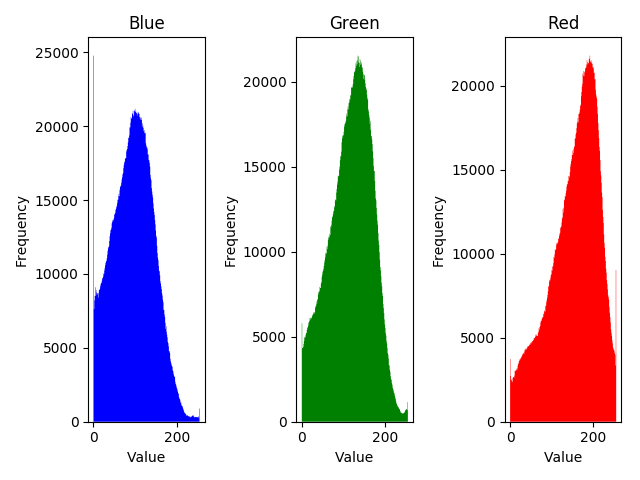
\includegraphics[width=2.5in]{../output/f_train_rgb_distributions.png}
\end{minipage}%
\begin{minipage}{0.5\linewidth}
\captionof{figure}{HSV distribution of female training images} \label{fig: hsv}
\centering
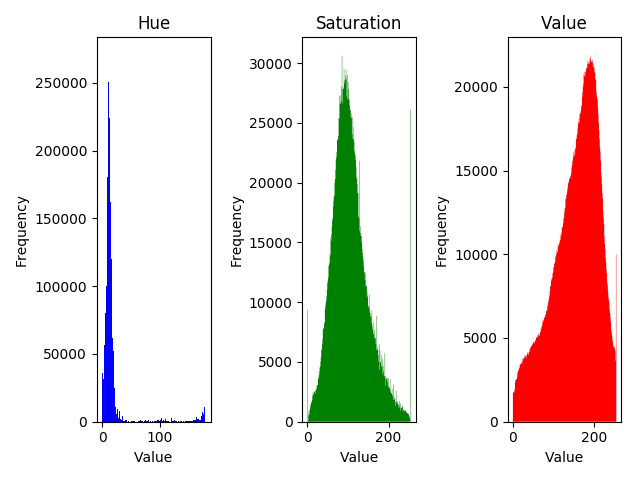
\includegraphics[width=2.5in]{../output/f_train_hsv_distributions.png}
\end{minipage}

\begin{minipage}{0.5\linewidth}
\captionof{figure}{HSV distribution of female training images} \label{fig: hsv_bad}
\centering
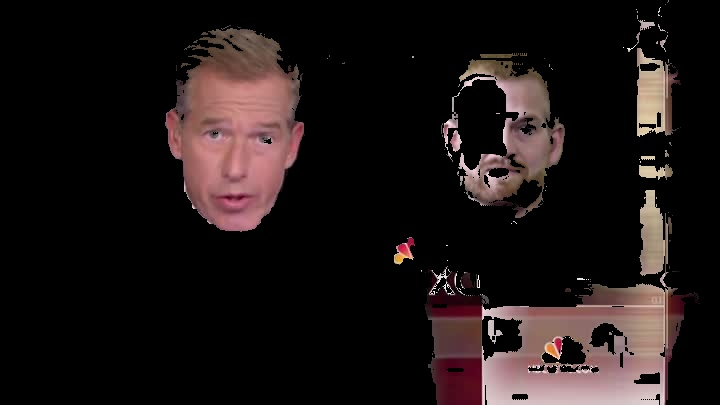
\includegraphics[width=2.5in]{../output/clip_1_hsv/050.jpg}

\end{minipage}%
\begin{minipage}{0.5\linewidth}
\captionof{figure}{HSV distribution of female training images} \label{fig: hsv_good}
\centering
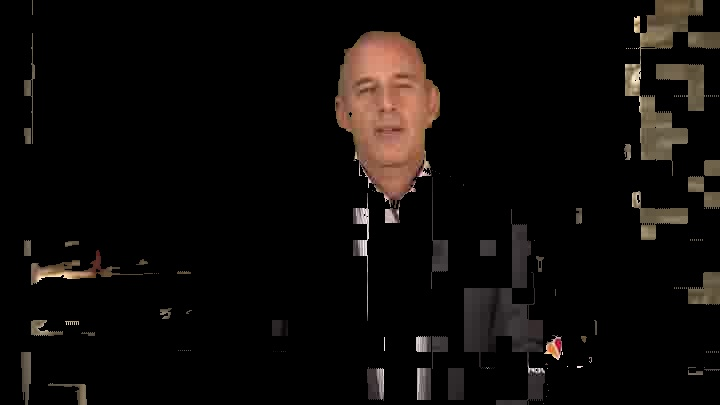
\includegraphics[width=2.5in]{../output/clip_1_hsv/160.jpg}
\end{minipage}

\section{Gender classification}
90\% of the images were used for training, whereas the other 10\% were used for testing the accuracy of the model.

\begin{minted}[bgcolor=bg]{sh}
python3 run.py train -m <model path>
\end{minted}

\begin{minted}[bgcolor=bg]{sh}
python3 run.py predict -m <model path>
\end{minted}

\subsection*{SVM}
For each detected face, the SIFT descriptors were extracted and fed to the trained SVM model. Then, a prediction for each descriptor is obtained. If there are more descriptors predicted as female, the 

\subsection*{Performance}
Table \ref{tab:gender_classification} shows the test accuracies of the three models. 

\begin{table}
 \caption{Gender classification performance}
  \centering
  \begin{tabular}{lll}
    \toprule
    Model		& Description		& Test accuracy \\
    \midrule
    SVM			& Input terminal	& 95.43\%     \\
    \bottomrule
  \end{tabular}
  \label{tab:gender_classification}
\end{table}

\section{References}
\href{https://www-nlpir.nist.gov/projects/tvpubs/tvpapers03/ramonlull.paper.pdf}{Video shot boundary detection based on color histogram}

\href{https://en.wikipedia.org/wiki/Shot_transition_detection}{Wikipedia - Shot transition detection}

\end{document}